\documentclass[11pt]{article}
\usepackage[margin=0.86in]{geometry}
\usepackage[T1]{fontenc}
\usepackage[utf8]{inputenc}
\usepackage{lmodern}
\usepackage{microtype}
\usepackage{graphicx}
\usepackage{booktabs}
\usepackage{array}
\usepackage{longtable}
\usepackage{multirow}
\usepackage{amsmath,amssymb}
\usepackage{siunitx}
\usepackage{xcolor}
\usepackage{authblk}
\usepackage{enumitem}
\usepackage{caption}
\usepackage{subcaption}
\usepackage{hyperref}
\usepackage[backend=biber,style=numeric-comp,sorting=none,maxbibnames=8]{biblatex}
\addbibresource{references.bib}

\hypersetup{colorlinks=true,linkcolor=blue!55!black,citecolor=blue!55!black,urlcolor=blue!55!black,pdfauthor={Eva Paunova},pdftitle={Round-Aware Validation and Constraint-Aware Ranking for AI-Guided Cell-Culture Media Development}}
\setlength{\parskip}{0.35em}
\setlength{\parindent}{0pt}
\captionsetup{font=small,labelfont=bf}
\renewcommand{\arraystretch}{1.15}
\newcommand{\kp}{\textit{K. phaffii}}
\newcommand{\pbmc}{PBMC}

\title{\textbf{Round-Aware Validation and Constraint-Aware Ranking for AI-Guided Cell-Culture Media Development: A Public-Data Benchmark}}
\author[1]{Eva Paunova\thanks{Correspondence: \href{mailto:eva@arcentlabs.com}{eva@arcentlabs.com}}}
\affil[1]{ArcentLabs, Europe}
\date{July 2026}

\begin{document}
\maketitle

\begin{abstract}
Artificial-intelligence-guided experimental design can reduce the number of wet-lab experiments required for cell-culture media development, yet evaluation practice has not kept pace with the sequential structure and multiple constraints of bioprocess optimization. Random cross-validation can mix observations acquired in later experimental rounds with earlier observations, producing estimates that are poorly aligned with prospective use. Furthermore, single-objective ranking can conceal unacceptable losses in viability, population balance, process burden, or product quality. We present a reproducible public-data benchmark that separates prediction from decision quality and evaluates models under three protocols: repeated random cross-validation, round-blocked validation, and forward-round prediction. We reanalyze openly released experiments spanning a four-component human peripheral-blood mononuclear-cell media blend (24 observations, four rounds), a four-factor \kp{} production task (86 observations, seven rounds plus 16 held-out validation conditions), and a nine-factor \kp{} task (77 observations, seven rounds). Ridge regression, random forests, and extremely randomized trees are compared with a mean baseline. Protocol choice materially changes error estimates and, in some tasks, model ranking. For the PBMC blend, the best random-CV RMSE was 14.79 percentage points, increasing to 18.17 under round-blocked and 18.60 under forward-round evaluation. In the four-factor \kp{} task, a ridge model achieved Spearman $\rho=0.75$ on the 16 held-out conditions but negative $R^2$, demonstrating useful ordering with weak absolute transfer. A non-compensatory homeostasis score independently recovers cytokine formulation 11 as the balanced PBMC candidate across a twofold tolerance sensitivity range. An illustrative Pareto analysis retains six efficient productivity--process-load trade-offs rather than a single optimum. The benchmark supports a practical standard: media-development models should be evaluated prospectively by experimental round, report ranking and calibration separately from point error, and preserve hard biological and process constraints during candidate selection.
\end{abstract}

\textbf{Keywords:} cell-culture media; active learning; Bayesian optimization; bioprocess development; round-aware validation; multi-objective optimization; uncertainty; PBMC; \kp{}

\section{Introduction}
Cell-culture media and feeding strategies determine whether a production host grows, remains viable, preserves the desired phenotype, and generates a product at acceptable yield and quality. The design space may combine basal media, nutrients, carbon sources, growth factors, cytokines, trace elements, pH, temperature, and time-varying feeds. These factors interact nonlinearly, while experiments are expensive and often constrained by material availability. Conventional one-factor-at-a-time and response-surface workflows therefore face a combinatorial and model-mismatch problem as the number of factors increases \cite{zhou2023,combe2021}.

Active learning and Bayesian optimization (BO) address this problem by fitting a surrogate model, balancing exploration and exploitation, and selecting the next experimental batch \cite{rasmussen2006,jones1998,hie2020}. Recent biological demonstrations include mammalian medium optimization with gradient-boosted trees \cite{hashizume2023}, multi-information-source and multi-objective optimization for cellular agriculture \cite{cosenza2022,cosenza2023}, and iterative optimization of PBMC culture and recombinant-protein production in \kp{} \cite{narayanan2025}. Hybrid models can additionally encode mass balances or mechanistic structure instead of asking a data-driven model to relearn known process constraints \cite{raissi2019,cui2023}.

Two gaps remain important for translation. First, sequential experimental datasets are not exchangeable. An observation acquired in round six was proposed using information unavailable in round zero. Randomly mixing rounds during cross-validation can therefore answer an easier retrospective question than the prospective one faced by a bioprocess scientist: \emph{how well will the current model rank the next experimental batch?} Structured validation is well established for temporal and hierarchical data \cite{roberts2017,vabalas2019}, but has not been standardized for cell-culture media optimization.

Second, a high value for one objective can compensate numerically for a biologically unacceptable result in another. A weighted average may rank a formulation with high productivity but poor viability above a safe formulation, unless weights and constraints are specified carefully. Media development is naturally non-compensatory: a failed sterility, viability, phenotype, metabolite, osmolality, or quality constraint should not disappear inside a favorable mean score.

Here, we introduce a public-data benchmark focused on these two gaps. We do not propose a new wet-lab optimum or claim host-agnostic generalization. Instead, we contribute: (i) three reproducible prediction tasks reconstructed from public iterative experiments; (ii) random, round-blocked, and forward-round validation; (iii) transparent linear and tree-ensemble baselines; (iv) held-out validation separating ranking from absolute prediction; and (v) non-compensatory and Pareto candidate-ranking examples. Figure~\ref{fig:workflow} summarizes the intended use.

\begin{figure}[t]
\centering
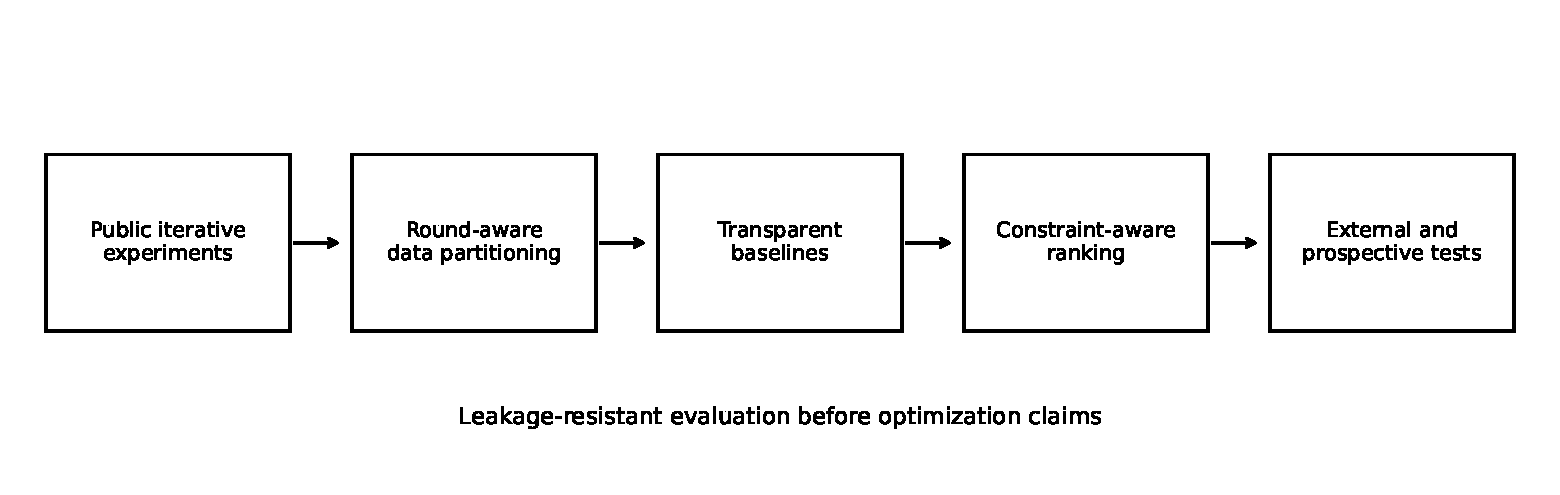
\includegraphics[width=0.98\linewidth]{../figures/benchmark_workflow.pdf}
\caption{Benchmark workflow. Public sequential experiments are partitioned by experimental round, evaluated with transparent baselines, and passed to constraint-aware candidate ranking. External and prospective tests are treated as distinct from retrospective random cross-validation.}
\label{fig:workflow}
\end{figure}

\section{Data and benchmark tasks}
\subsection{Public source and scope}
All empirical analyses use the source-data workbook released with Narayanan \textit{et al.} \cite{narayanan2025}. The original article and source data are available under CC BY 4.0, and the authors also provide formulations through Figshare and code through GitHub and Zenodo. We extracted tabular values required for the analyses and provide machine-readable derivative CSV files with attribution. No private, clinical, proprietary-media, or newly generated wet-lab data are used.

Table~\ref{tab:tasks} defines the benchmark tasks. The primary endpoints are average PBMC viability after culture and specific productivity for \kp{} cultures. Experimental round is retained as a first-class variable for evaluation but is not supplied as a predictor.

\begin{table}[ht]
\centering
\caption{Public benchmark tasks reconstructed from the source-data workbook.}
\label{tab:tasks}
\small
\begin{tabular}{p{2.5cm}rrp{3.4cm}p{3.35cm}}
\toprule
Task & $n$ & Rounds & Inputs & Endpoint \\
\midrule
PBMC media blend & 24 & 4 & Fractions of DMEM, RPMI-10, XVIVO, and AR5 & Average viability (\%) \\
\kp{} four-factor & 86 & 7 & Carbon-source identity, carbon concentration, glycerol, methanol & Specific productivity (mg L$^{-1}$ OD$_{600}^{-1}$) \\
\kp{} four-factor external set & 16 & -- & Same four inputs; not used for model fitting & Specific productivity \\
\kp{} nine-factor & 77 & 7 & Carbon source plus eight continuous medium/process factors & Specific productivity \\
PBMC cytokine ranking & 12 & 2 & Cytokine formulations; output-only secondary analysis & Total viability and B-, NK-, and T-cell changes \\
\bottomrule
\end{tabular}
\end{table}

\subsection{PBMC media-blend task}
The PBMC study optimized a convex blend of four commercial media, whose fractions sum to approximately 100\%. Twenty-four experiments were executed in four batches of six. The endpoint is mean viability across available biological measurements. The small sample size makes this task intentionally difficult and highlights how uncertainty in a prospective setting differs from a randomly shuffled estimate.

\subsection{Four-factor and nine-factor \kp{} tasks}
The four-factor task combines a categorical carbon source with carbon concentration, glycerol percentage, and methanol percentage. Eighty-six observations from rounds 0--6 form the development set. Sixteen conditions labelled as validation in the public workbook are held out completely until final evaluation. The nine-factor task adds glutathione and Tween variables for outgrowth and production, plus pH, yielding 77 observations over seven rounds. These two tasks test increasing dimensionality without claiming transfer across biological hosts.

\subsection{PBMC cytokine homeostasis task}
A separate public experiment measured the change in total cell viability and in B-cell, NK-cell, and T-cell abundance for 12 cytokine formulations. The source study identified formulation 11 as meeting the desired objective \cite{narayanan2025}. We use these outputs only to test whether a generic non-compensatory score identifies the same balanced candidate without fitting a predictive model.

\subsection{Roadmap to industrial mammalian hosts}
The public benchmark is not a substitute for CHO or HEK293 process-development data. A future host-transfer benchmark should include harmonized media composition, feed timing, viable-cell density, metabolite trajectories, titer, and critical-quality attributes. GSE30321 provides 295 CHO microarrays from 121 cultures and nine process variables across media, feed, scale, temperature, duration, and product conditions \cite{gse30321,clarke2011}. PXD018439 provides time-resolved CHO-K1 fed-batch proteomics \cite{pxd018439}. These resources support representation and response-model research, but incomplete or proprietary media composition prevents a clean host-agnostic media-optimization claim from the present analysis.

\section{Methods}
\subsection{Preprocessing and baseline models}
Continuous inputs were standardized for ridge regression. Carbon-source identity was one-hot encoded with an unknown-category fallback. We evaluated a mean predictor, ridge regression \cite{hoerl1970}, random forests \cite{breiman2001}, and extremely randomized trees \cite{geurts2006}. Tree ensembles used 150 estimators, minimum leaf size 2, and 0.8 feature subsampling. All stochastic components used seed 2026. Implementations use scikit-learn \cite{pedregosa2011}.

These baselines deliberately avoid extensive hyperparameter search. On small iterative datasets, nested tuning can consume substantial degrees of freedom and may obscure the larger effect of partition design. The benchmark is intended as a minimum reporting standard rather than a leaderboard optimized to the current dataset.

\subsection{Three validation protocols}
Let $D_r=\{(x_i,y_i): g_i=r\}$ denote observations from experimental round $r$. We compare:

\begin{enumerate}[leftmargin=1.5em]
\item \textbf{Repeated random CV:} four-fold CV repeated three times. Rounds are mixed across training and test partitions.
\item \textbf{Round-blocked validation:} leave-one-round-out. Each complete experimental batch is tested after fitting on all other rounds.
\item \textbf{Forward-round validation:} for each $r>0$, fit only on $\cup_{k<r}D_k$ and test on $D_r$.
\end{enumerate}

Forward-round validation is closest to prospective operation, whereas round-blocked validation quantifies batch sensitivity without preserving temporal order. We report fold-level mean and standard deviation of mean absolute error (MAE), root mean squared error (RMSE), Spearman rank correlation, and $R^2$. For cross-task visualization, RMSE is normalized by the sample standard deviation of the task endpoint.

\subsection{External validation}
For the four-factor \kp{} task, models are fitted once on all 86 development observations and evaluated on the 16 conditions explicitly labelled as validation in the workbook. We separately interpret point accuracy and rank correlation. A model can rank candidates usefully while remaining poorly calibrated in absolute units; conversely, a small average error may not guarantee correct ordering of the best candidates.

\subsection{Non-compensatory biological ranking}
For cytokine formulation $x$, let $d_j(x)$ be the change from the desired baseline for endpoint $j\in\{\text{total},B,NK,T\}$. We transform each deviation to utility
\begin{equation}
 u_j(x)=\exp\left(-\frac{|d_j(x)|}{\tau_j}\right),
\end{equation}
where $\tau_j$ is the 75th percentile of $|d_j|$ across tested formulations. The non-compensatory score is
\begin{equation}
 S_{\min}(x)=\min_j u_j(x).
\label{eq:minscore}
\end{equation}
A high value requires acceptable performance in every measured dimension. We vary all $\tau_j$ together from $0.5\times$ to $2\times$ their nominal values to test ranking sensitivity. This score is an illustrative decision rule, not a clinical threshold.

\subsection{Illustrative resource-aware Pareto ranking}
The public workbook does not provide monetary cost, osmolality, raw-material sustainability, or mixing constraints. To illustrate multi-objective reporting without inventing such quantities, we define a transparent process-load proxy for the four-factor \kp{} task:
\begin{equation}
 C(x)=\frac{1}{3}\sum_{k\in\{c,g,m\}}\frac{x_k-\min(x_k)}{\max(x_k)-\min(x_k)},
\end{equation}
where $c$, $g$, and $m$ denote carbon concentration, glycerol, and methanol. We identify nondominated candidates that maximize measured specific productivity and minimize $C(x)$. This proxy is not a cost model and should not be used to select a manufacturing condition without domain-specific constraints.

\section{Results}
\subsection{Iterative experiments improve observed outcomes but do not ensure predictive transfer}
Figure~\ref{fig:progression} shows median and best observed outcomes by experimental round, normalized separately within each task for visualization. The PBMC blend displays a clear improvement in the final round, with mean viability increasing from 39.98\% in round 0 to 72.65\% in round 3. In the four-factor \kp{} task, median specific productivity increased from 2.38 in round 0 to 9.48 in round 5, while the best observed value reached 12.35. The nine-factor task also shifted toward higher outcomes in later rounds, but with non-monotonic batch means. These trajectories demonstrate successful exploration of better regions; they do not, by themselves, establish generalization to unseen rounds or hosts.

\begin{figure}[ht]
\centering
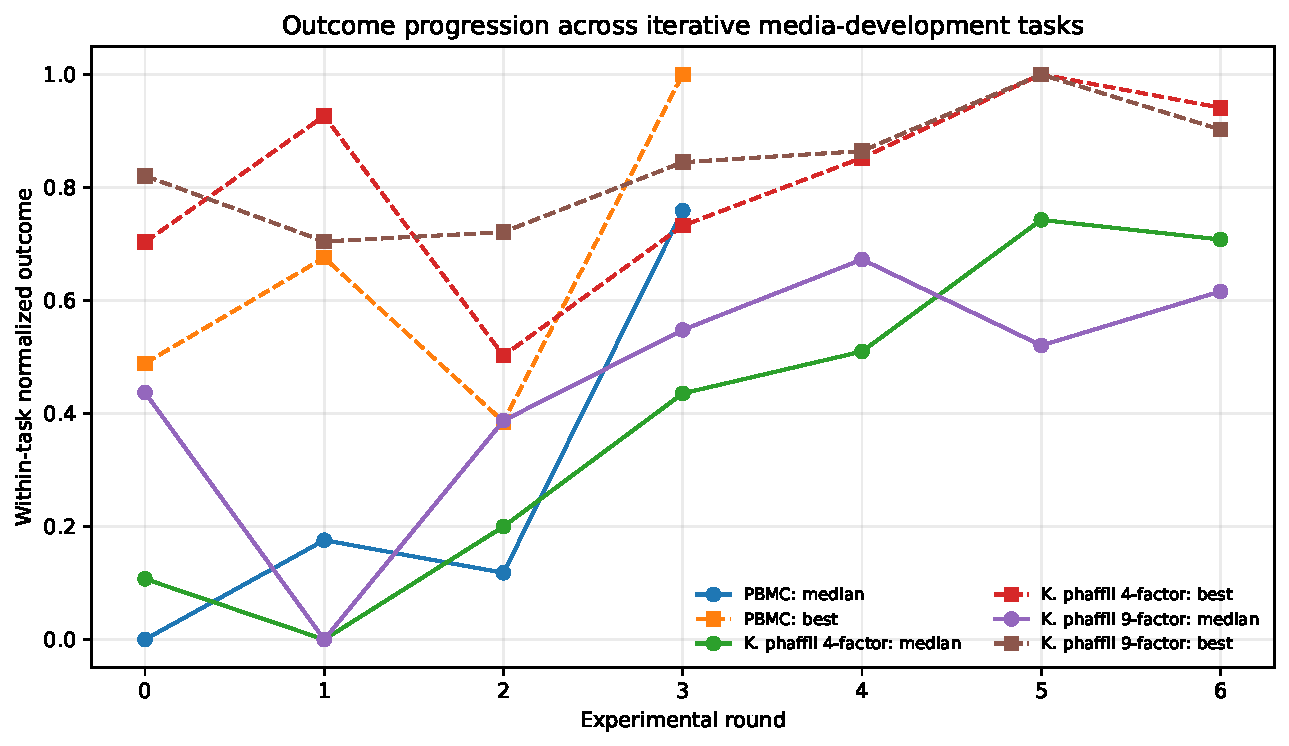
\includegraphics[width=0.88\linewidth]{../figures/round_progression.pdf}
\caption{Within-task normalized median and best outcome by experimental round. Normalization is used only to display endpoints with different units on one axis. Raw values are provided in the reproducibility package.}
\label{fig:progression}
\end{figure}

\subsection{Validation protocol changes reported performance and model selection}
Table~\ref{tab:rmse} and Figure~\ref{fig:heatmap} summarize RMSE. In the PBMC task, extremely randomized trees had the lowest random-CV RMSE (14.79 percentage points), but error increased by 22.9\% under round-blocked validation and 25.8\% under forward-round validation. The random forest showed a similar increase. The apparent advantage over the mean baseline narrowed substantially when complete future batches were withheld.

For the four-factor \kp{} task, extremely randomized trees remained the strongest baseline by RMSE, but forward-round error (2.17) exceeded random-CV error (1.91). In the nine-factor task, model ranking was protocol-dependent: extremely randomized trees were best under random CV, whereas random forests were marginally better under round-blocked and forward-round evaluation. Thus, the choice of split can influence not only the estimated error but also the algorithm selected for deployment.

\begin{table}[ht]
\centering
\caption{Fold-mean RMSE under three validation protocols. Lower is better. Units follow each task endpoint.}
\label{tab:rmse}
\small
\begin{tabular}{llrrr}
\toprule
Task & Model & Random CV & Round-blocked & Forward-round \\
\midrule
\multirow{4}{*}{PBMC}
 & Mean & 17.93 & 19.90 & 19.55 \\
 & Ridge & 20.09 & 21.80 & 20.21 \\
 & Random forest & 15.83 & 19.40 & 20.15 \\
 & Extra trees & \textbf{14.79} & \textbf{18.17} & \textbf{18.60} \\
\midrule
\multirow{4}{*}{\kp{} 4-factor}
 & Mean & 3.50 & 3.76 & 3.93 \\
 & Ridge & 2.04 & 2.15 & 2.34 \\
 & Random forest & 2.26 & 2.29 & 2.66 \\
 & Extra trees & \textbf{1.91} & \textbf{1.84} & \textbf{2.17} \\
\midrule
\multirow{4}{*}{\kp{} 9-factor}
 & Mean & 3.42 & 3.49 & 3.46 \\
 & Ridge & 3.00 & 3.40 & 3.09 \\
 & Random forest & 2.88 & \textbf{2.81} & \textbf{2.71} \\
 & Extra trees & \textbf{2.77} & 2.85 & 2.73 \\
\bottomrule
\end{tabular}
\end{table}

\begin{figure}[ht]
\centering
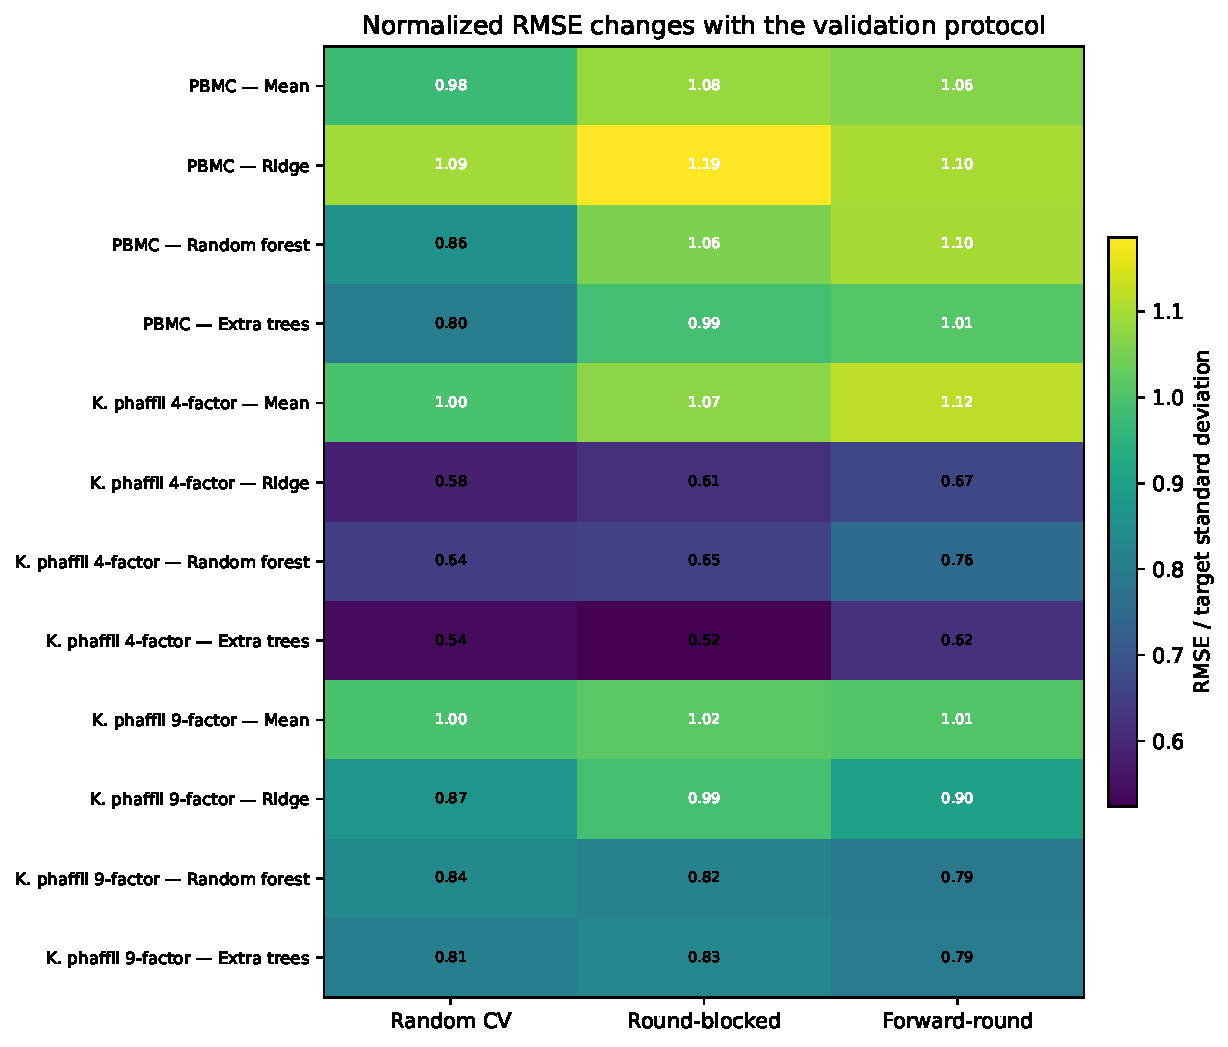
\includegraphics[width=0.88\linewidth]{../figures/protocol_nrmse_heatmap.pdf}
\caption{Normalized RMSE by task, model, and validation protocol. Values are fold-mean RMSE divided by the endpoint standard deviation. Random splits can yield materially different estimates from batch-blocked and forward-round tests.}
\label{fig:heatmap}
\end{figure}

\subsection{Held-out conditions separate useful ranking from absolute calibration}
Table~\ref{tab:external} reports performance on the 16 held-out four-factor conditions. Ridge achieved $\rho=0.75$ and extra trees $\rho=0.60$, indicating that relative ordering was partially transferable. However, all models had negative $R^2$, including ridge ($-0.19$) and extra trees ($-0.21$). Figure~\ref{fig:external} shows systematic deviations from the identity line. This result cautions against treating a rank-capable surrogate as an accurate digital representation of absolute process response.

\begin{table}[ht]
\centering
\caption{External validation on 16 four-factor \kp{} conditions.}
\label{tab:external}
\small
\begin{tabular}{lrrrr}
\toprule
Model & MAE & RMSE & Spearman $\rho$ & $R^2$ \\
\midrule
Mean & 2.42 & 2.98 & -- & $-0.85$ \\
Ridge & 1.85 & \textbf{2.39} & \textbf{0.75} & $-0.19$ \\
Random forest & 2.31 & 2.94 & 0.36 & $-0.79$ \\
Extra trees & \textbf{1.83} & 2.41 & 0.60 & $-0.21$ \\
\bottomrule
\end{tabular}
\end{table}

\begin{figure}[ht]
\centering
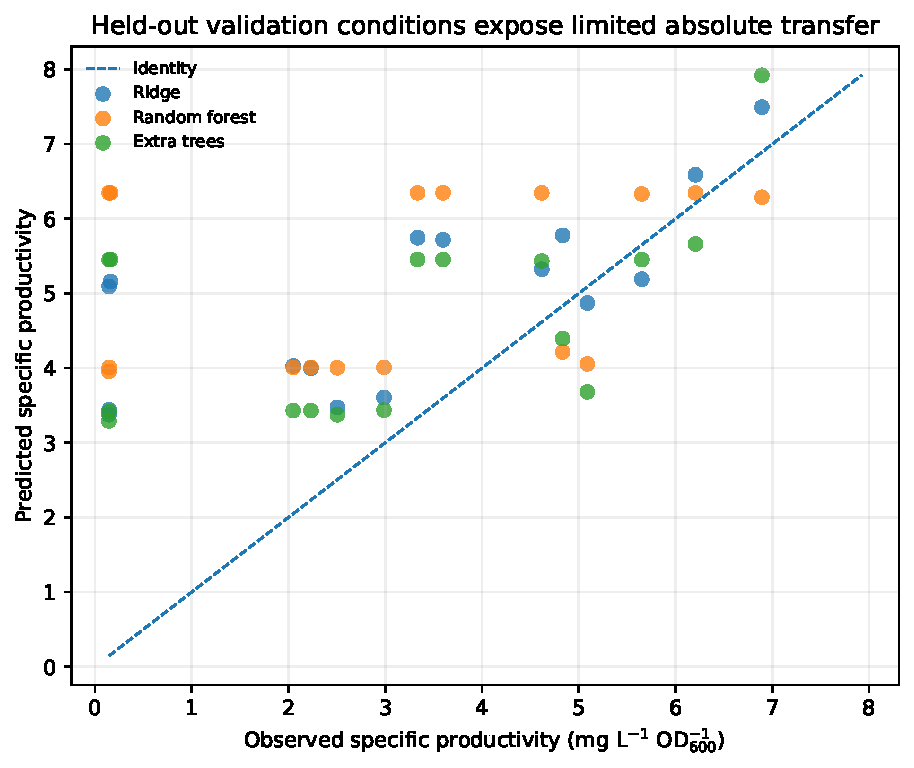
\includegraphics[width=0.72\linewidth]{../figures/external_validation.pdf}
\caption{Observed versus predicted productivity for held-out four-factor conditions. The dashed line is identity. Rank correlation is moderate for ridge and extra trees, while negative $R^2$ indicates weak absolute transfer.}
\label{fig:external}
\end{figure}

\subsection{Non-compensatory ranking identifies a balanced PBMC formulation}
Equation~\ref{eq:minscore} assigned the highest worst-dimension utility to formulation 11 ($S_{\min}=0.815$), followed by formulation 10 (0.587) and formulation 5 (0.396). Formulation 11 had changes of 12.6\% in total viability, 0.71\% in B cells, $-4.24$\% in NK cells, and 3.40\% in T cells. It remained the top-ranked formulation for every common tolerance multiplier between 0.5 and 2.0. This independently recovers the balanced condition highlighted by the source experiment while making the decision rule explicit (Figure~\ref{fig:homeostasis}).

\begin{figure}[ht]
\centering
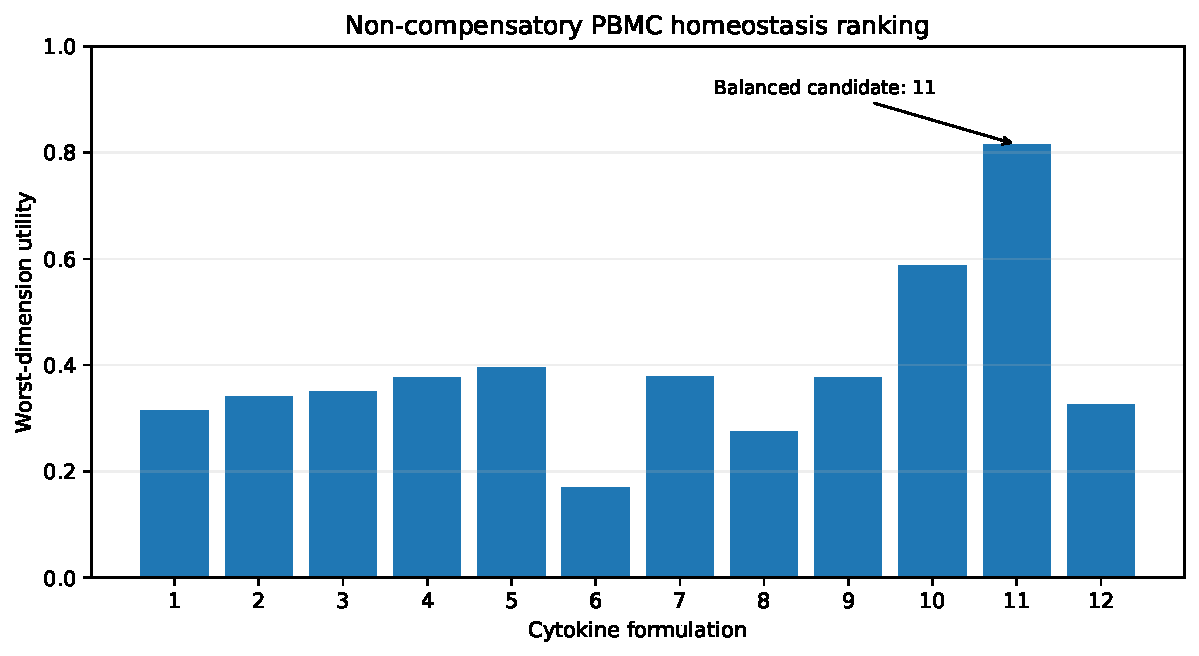
\includegraphics[width=0.84\linewidth]{../figures/pbmc_noncompensatory_score.pdf}
\caption{Worst-dimension utility for 12 PBMC cytokine formulations. A high score requires simultaneously small deviations in total viability and B-, NK-, and T-cell measurements.}
\label{fig:homeostasis}
\end{figure}

\subsection{Pareto reporting avoids a false single optimum}
Six measured four-factor media were nondominated for productivity and the illustrative process-load proxy (Figure~\ref{fig:pareto}). The frontier ranged from a low-load glycerol condition with productivity 6.88 and proxy 0.007 to a galactose condition with productivity 12.35 and proxy 0.211. Between these extremes, several formulations offered substantial productivity gains for small increments in the proxy. The result is not a manufacturing recommendation; it demonstrates why optimization reports should show trade-offs and allow decision makers to apply actual cost, safety, solubility, and quality constraints.

\begin{figure}[ht]
\centering
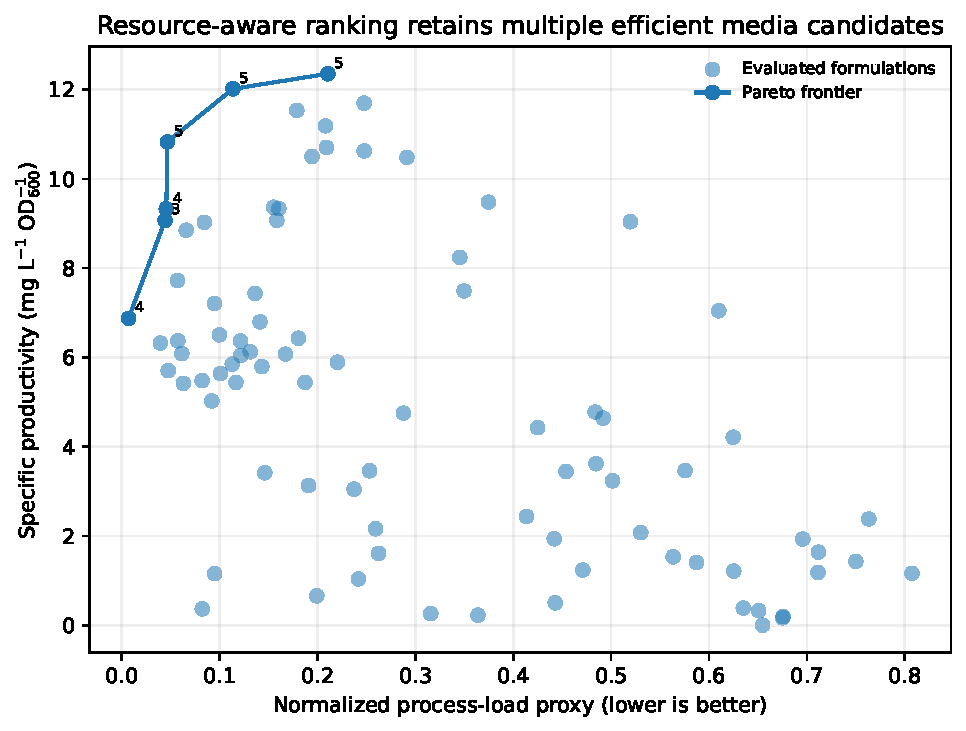
\includegraphics[width=0.76\linewidth]{../figures/kp4_pareto.pdf}
\caption{Measured specific productivity versus an illustrative normalized process-load proxy. The connected points are nondominated. Labels indicate experimental round. The proxy is not monetary cost and excludes product-quality constraints.}
\label{fig:pareto}
\end{figure}

\section{Discussion}
The benchmark suggests that evaluation design is a first-order component of AI-assisted media development. Random CV remains useful for debugging and model comparison under an interpolation assumption, but it should not be the sole evidence for prospective deployment. Forward-round validation directly simulates the repeated cycle of model fitting, candidate selection, and wet-lab testing. Round-blocked validation adds a stress test for batch sensitivity. Reporting all three reveals whether an apparent gain is robust to sequential structure.

The held-out \kp{} experiment further shows why point prediction and decision quality should be separated. A rank correlation of 0.75 may support shortlist construction, but negative $R^2$ argues against interpreting the same model as an accurate quantitative simulator. For operational use, uncertainty intervals, calibration diagnostics, applicability-domain checks, and abstention rules should accompany candidate ranks. The next experiment should not be selected solely because it has the highest predicted mean; it should also satisfy hard constraints and have an uncertainty profile appropriate to the decision.

The non-compensatory PBMC analysis formalizes a principle common in bioprocessing: a candidate is only as deployable as its most important failed requirement. A minimum utility is intentionally conservative. Other choices include lexicographic constraints, chance constraints, constrained expected improvement, or Pareto-front selection. The important point is that biological and process requirements should remain visible rather than being hidden inside an undocumented weighted sum.

A genuinely host-agnostic model remains a longer-term target. Transfer across PBMCs, yeast, CHO, and HEK293 cannot be inferred from a pooled table of heterogeneous experiments. Such a model would require a shared representation of medium chemistry, host metabolism, process state, measurement protocol, and product objective. Mechanistic mass balances and metabolic constraints can provide common structure, while a learned residual captures host- and product-specific effects. The correct evaluation would leave out entire hosts, cell lines, products, or laboratories, not only individual rows.

\section{Limitations}
The study is a secondary analysis of a single public experimental program. Sample sizes are small, rounds were generated adaptively, and the factors differ between tasks. The random, blocked, and forward protocols therefore estimate performance for these datasets rather than a universal ranking of algorithms. Fold-level Spearman estimates are unstable when a round contains only six observations, so RMSE and external-set ranking receive greater emphasis.

The external set is limited to 16 four-factor conditions and does not constitute independent multi-laboratory validation. The process-load proxy omits actual raw-material price, osmolality, solubility, environmental impact, feed timing, and product quality. The PBMC utility tolerances are empirical scale parameters rather than clinical specifications. No causal or mechanistic claim is made from feature-response associations. Finally, this benchmark does not analyze proprietary CHO or HEK293 media and cannot establish host-agnostic optimization.

\section{Reproducibility, data, and code}
The reproducibility package contains derivative CSV files, a deterministic Python script, environment requirements, flat metric tables, figure-generation code, and the full result summary in JSON. The raw source workbook is publicly available with the original article \cite{narayanan2025}. Derived data retain source attribution. The analysis script reconstructs all figures and reported numerical results using seed 2026.

\section{Conclusion}
AI can accelerate cell-culture media and process development only when model evaluation matches the way experiments are actually conducted. Across public PBMC and \kp{} experiments, forward-round and round-blocked evaluation changed error estimates and sometimes changed the preferred model. Held-out validation revealed that useful ranking can coexist with poor absolute calibration. Non-compensatory and Pareto reporting preserved biological balance and process trade-offs that a single scalar objective could conceal. We recommend that future studies report random, batch-blocked, and prospective validation; separate rank quality from absolute accuracy; publish applicability and uncertainty diagnostics; and enforce hard biological, quality, and process constraints before proposing wet-lab candidates.

\section*{Ethics statement}
No new human-participant or animal experiments were performed. The work is a secondary computational analysis of publicly released aggregate experimental data. Readers should consult the source study for its ethics and sample-governance statements.

\section*{Author contributions}
E.P. conceived the benchmark, designed the analyses, interpreted the results, and prepared the manuscript and reproducibility package.

\section*{Funding}
This research received no external funding.

\section*{Competing interests}
E.P. is the founder of ArcentLabs. No commercial product, proprietary medium, or paid service was evaluated in this study.

\section*{Use of generative AI}
Generative-AI tools were used for language editing and code scaffolding. The author is responsible for verification of the analyses, references, and final manuscript.

\printbibliography
\end{document}
